\documentclass[10pt,a4paper]{article}

\usepackage[margin=1.65cm,top=1.4cm,bottom=1.5cm]{geometry}
\usepackage{amsmath,amssymb}
\usepackage{graphicx}
\usepackage{booktabs}
\usepackage{xcolor}
\usepackage[hidelinks]{hyperref}
\usepackage{caption}
\usepackage{titlesec}

\captionsetup{font=small,labelfont=bf,skip=2pt}
\titleformat{\section}{\normalfont\bfseries}{\thesection}{0.6em}{}
\titlespacing*{\section}{0pt}{5pt}{1pt}
\setlength{\parskip}{2.5pt plus 1pt}
\setlength{\parindent}{0pt}
\setlength{\abovedisplayskip}{3pt}\setlength{\belowdisplayskip}{3pt}
\setlength{\abovedisplayshortskip}{1pt}\setlength{\belowdisplayshortskip}{2pt}
\setlength{\textfloatsep}{6pt plus 2pt}

\newcommand{\code}[1]{\texttt{#1}}
\newcommand{\topk}{\operatorname{TopK}}
\newcommand{\PH}[1]{\textcolor{red}{[#1]}}

\begin{document}

{\centering
{\large\bfseries RBLapSum in a 24-layer code-residual stack: why it collapses, and a first-order surrogate that trains}\\[1pt]
{\small TinyStories; \(d=1024\), \(N=4096\), \(K=32\), \(J=224\), \(T=1\), \code{through\_rank\_kappa}, MD optimizer,
lr \(3\!\cdot\!10^{-4}\).  Full record, all runs and negative results: \code{docs/rblapsum-code-residual-journal.tex}.}\par}

\section{Observation}

The code residual (\code{docs/stream-bottleneck-depth.tex}) makes a 24-layer stream-bottleneck model train with
hard \(\topk\): block \(\ell\) reads the \(K\)-sparse code through the decoder and only its contribution is encoded,
\begin{equation*}
  c_{\ell+1}=\topk(u_\ell),\qquad u_\ell=c_\ell+v_\ell,\qquad v_\ell=W_E\,\Delta_\ell(g_DW_Dc_\ell).
\end{equation*}
RBLapSum keeps the hard forward and adds a support term to the backward, which lets the \(J\) next candidates move.
With scores \(s_i=|u_i|\), the rank boundary \(b=s_{(K+1)}\), the hard mask \(m\) and \(g=\partial\mathcal L/\partial c_{\ell+1}\),
\begin{equation}
  \frac{\partial\mathcal L}{\partial u_i}=m_ig_i+\gamma\,\operatorname{sign}(u_i)\Bigl(a_i-q_i\sum\nolimits_ja_j\Bigr),\qquad
  a_i=g_iu_i\kappa_i,\quad \kappa_i=\frac{e^{-|s_i-b|/T}}{2T},\quad q_i=\frac{\kappa_i}{\sum_j\kappa_j},
  \label{eq:rbk}
\end{equation}
summed over the Top-\((K+J)\) pool; \(\gamma\) is the support scale (\code{rblapsum\_support\_scale}, 1 by default).  In
the 24-layer code residual the unmodified surrogate fails: the gradient norm is \(1.2\cdot10^4\) from the first step
(hard: \(\sim\)1), by step 300 91--94\,\% of the features never enter any token's support, and validation CE is 5.31
at step 2000 against 2.104 for the exact hard backward (unigram entropy 5.97).

\section{First mechanism: support terms multiply along the carried code}

The carry is the identity on each code coordinate, so one gate's backward multiplies \(g_i\) by
\(m_i+\gamma|u_i|\kappa_i\), which is \(1+b/(2T)\approx3\) for an active feature at the boundary (\(b\approx4\) at
initialization).  The unmodified backward applies each gate's support term to the total upstream gradient, which
already contains the support terms of the gates above; for a feature that is carried near the boundary they multiply.
At initialization the gradient reaching the code grows \(\times1.67\) per block toward the input relative to the hard
model's, \(2.6\cdot10^5\) times the hard model's at the entry gate (Fig.~\ref{fig:mech}a).  A product of support terms at several gates is a term of
second or higher order in the changes of support: it describes several gates changing their support at once.  The
hard forward has no such terms; they are estimator error, not signal.  Smoothing the forward does not remove them:
the soft gate \(u\mapsto u\,p\bigl((|u|-b)/T\bigr)\) has slope \(p+|u|\kappa>1\) near the boundary, and its exact
gradient grows \(\times1.4\) per block relative to the hard model's.  A larger \(T\) lowers \(\kappa\) at the boundary but
spreads it over more of the pool (still \(\times1.2\) per block at \(T=16\)).

\section{Routing the term past the carry: one input, two gradients}

The obvious repair routes the support term only into the block's update: \(\partial\mathcal L/\partial c_\ell=m\odot g\)
and \(\partial\mathcal L/\partial v_\ell=m\odot g+D_\ell^\top g\), with \(D_\ell^\top g\) the support term of
\eqref{eq:rbk} (scope \code{update}).  It removes the products
(\(\times1.07\) per block at initialization, against \(\times1.67\)), but training still collapses, more slowly: dead features from
step 200, val CE 5.96 at step 2000.  The code at every gate is then held by \(K\) features that are active for more
than half of the tokens; they carry 91--95\,\% of the code's energy and the codes of all positions nearly coincide
(Fig.~\ref{fig:mech}b; the common-mode fraction \(f\) of the code within a sequence is 0.81--0.86).  With \(K\) slots
held by token-independent features the readout sees only the unigram.  The hard backward forms such features only at
the last gate while it learns the unigram (60--69\,\% of that gate's energy at steps 50--100) and dissolves them by
step 600; under the routed surrogate they spread down to gate 6 by step 200 and to every gate by step 450.  Of the
routed term, the part on active features is the destructive one (73\,\% dead features by step 1000, against 1\,\% with
the inactive part alone).

Routing violates a requirement that any estimator of this stack's gradient must meet: \(c_\ell\) and \(v_\ell\) enter
the gate only through their sum, so they must receive the same gradient.  Under the routing the carry gets the
exact \(m\odot g\) and the update the support term on top: at the boundary block \(\ell\) learns the values of its
marginal features about three times faster than the blocks that wrote them, i.e.\ the parameters are trained on two
different estimates of the same derivative.  Two requirements follow, and neither variant meets both:
\textbf{(R1)} one gradient for the gate's input \(u_\ell\) (the routing violates it); \textbf{(R2)} no products of support
terms (the unmodified backward violates it).

\section{Fix: the first-order estimator}

Write the RBLapSum Jacobian of gate \(\ell\) as \(M_\ell+D_\ell\): the hard mask plus the support term.  The
unmodified backward is the backward pass of a stack in which every gate uses \(M_\ell+D_\ell\) at once; along the
carried code it multiplies \(\prod_\ell(M_\ell+D_\ell)\), whose terms with two or more \(D\)'s grow as \((1+b/2T)^n\).  The single-gate
surrogate, which is what RBLapSum was designed and tuned as, relaxes one gate and keeps the others exact.  Summing
it over the gates gives, with \(\partial\tilde{\mathcal L}_\ell/\partial\theta\) the backward pass in which only gate
\(\ell\) uses \(M_\ell+D_\ell\) and every other gate its mask,
\begin{equation}
  \frac{\partial\mathcal L}{\partial\theta}+\sum_\ell\Bigl(\frac{\partial\tilde{\mathcal L}_\ell}{\partial\theta}-\frac{\partial\mathcal L}{\partial\theta}\Bigr)
  \;=\;J_{\rm hard}^\top g_{\rm out}
  \;+\;\sum_\ell\Bigl(\frac{\partial u_\ell}{\partial\theta}\Bigr)^{\!\top}_{\!\rm hard}D_\ell^\top H_\ell ,
  \label{eq:fo}
\end{equation}
where \(H_\ell\) is the gradient that reaches gate \(\ell\)'s output along hard paths only and every other Jacobian is the
hard one: the first-order estimate, one change of support at a time.  Each term is a backward pass through the gate's
input \(u_\ell\), so the carry and the update receive the same gradient (R1), and no path carries two support terms
(R2).
Scaling the support term by \(\gamma\) in the unmodified backward gives \(\prod(M+\gamma D)\): the hard gradient, plus
\(\gamma\) times the sum in \eqref{eq:fo}, plus terms of order \(\gamma^2\).  \code{rblapsum\_surrogate\_scope=first\_order} computes \eqref{eq:fo} with two backward passes per
micro-batch: a hard pass (\code{torch.autograd.grad} to the token embedding, so no parameter's \texttt{.grad} is
touched) in which every gate passes back \(m\odot g\) and keeps \(g=H_\ell\), then the ordinary pass, in which each gate
adds \(D_\ell^\top H_\ell\).  It costs about 45\,\% more per step (1.57 against 1.09\,s).  At initialization the gradient
reaching the code grows \(\times1.09\) per block relative to the hard model's: the additive sum of the later gates'
terms, not their product (Fig.~\ref{fig:mech}a).

\begin{figure}[t]
\centering
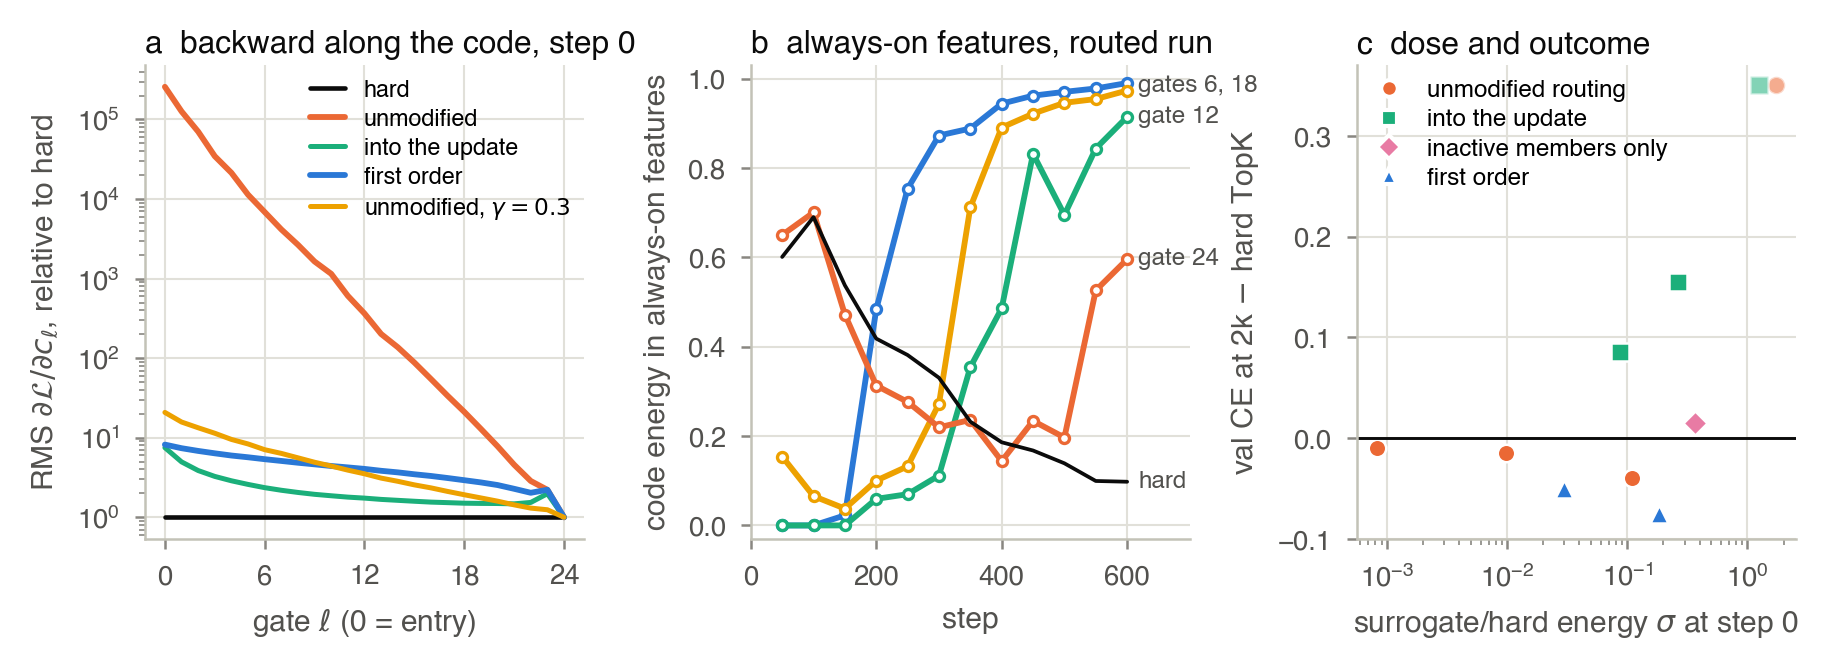
\includegraphics[width=\textwidth]{figures/surr/fig_mechanisms.png}
\caption{\textbf{a} Gradient reaching the carried code at initialization, relative to the hard model's.
\textbf{b} Share of the code's energy held by features active for more than half of the tokens, during the collapse
of the routed surrogate (one curve per gate) and for the hard backward (black, maximum over the gates).
\textbf{c} Surrogate energy at the gate at initialization (\(\lVert D^\top g\rVert^2/\lVert m\odot g\rVert^2\), mean over
gates) against validation CE at step 2000 minus the hard backward's; collapsed runs drawn at the top, faded.}
\label{fig:mech}
\end{figure}

\section{Results}

\begin{figure}[t]
\centering
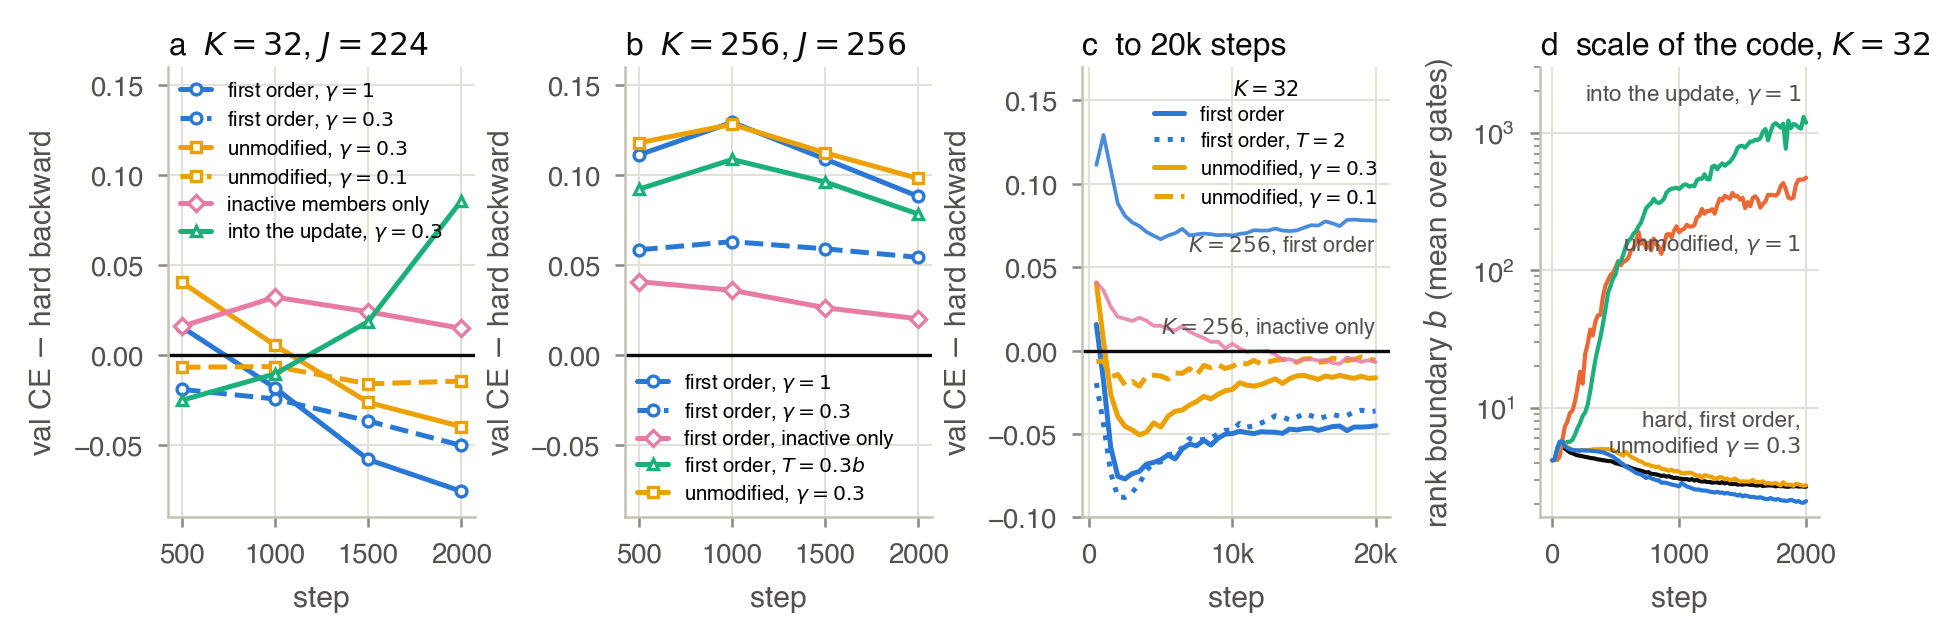
\includegraphics[width=\textwidth]{figures/surr/fig_training.png}
\caption{Training; \(\gamma\) is the support scale, \(T=1\).  \textbf{a} The 2000-step screens at \(K=32\), \(J=224\):
validation CE minus that of the exact hard backward (\(\gamma=0\)) of the same configuration.  \textbf{b} The same at
\(K=256\), \(J=256\).  \textbf{c} The runs continued to 20k steps, each against the hard backward of its own \(K\) (the
two \(K=256\) runs labelled).  \textbf{d} Rank boundary \(b\), the code's
scale at the boundary, mean over gates, \(K=32\).}
\label{fig:train}
\end{figure}

All runs: 24 layers, the same base configuration and seed; the hard reference is RBLapSum at \(\gamma=0\), the exact
hard backward on the same configuration.

\begin{center}\small
\begin{tabular}{lcccc}
\toprule
 & \(\sigma\), step 0 & per block, step 0 & val CE, step 2k & step 20k \\
\midrule
hard backward (\(\gamma=0\))                          & 0     & \(\times1.00\) & 2.104 & 1.502 \\
unmodified (\(\gamma=1\))                             & 1.72  & \(\times1.67\) & 5.314 & -- \\
unmodified, \(\gamma=0.3\)                            & 0.11  & \(\times1.13\) & 2.064 & 1.486 \\
unmodified, \(\gamma=0.1\)                            & 0.010 & \(\times1.03\) & 2.089 & 1.496 \\
unmodified, \(\gamma=0.03\)                           & 0.001 & \(\times1.01\) & 2.094 & -- \\
inactive members only (\(\gamma=1\))                  & 0.37  & \(\times1.02\) & 2.119 & -- \\
routed into the update (\(\gamma=1\))                 & 1.26  & \(\times1.07\) & 5.965 & -- \\
routed into the update, \(\gamma=0.3\)                & 0.087 & \(\times1.02\) & 2.189 & -- \\
\textbf{first order} (\(\gamma=1\))                   & 0.18  & \(\times1.09\) & \textbf{2.028} & \textbf{1.457} \\
first order, \(\gamma=0.3\)                           & 0.030 & \(\times1.05\) & 2.054 & -- \\
\bottomrule
\end{tabular}
\end{center}

\(\sigma\): surrogate/hard energy at the gate; per block: growth of the gradient reaching the code toward the input,
relative to the hard model.  At full strength the first-order estimator trains with no dead features and the
code's scale falling as in the hard model (Fig.~\ref{fig:train}d), and it is the best run from step 1000 on: 0.076 below
the hard backward at step 2000, against 0.040 for the best rescaling of the unmodified backward (\(\gamma=0.3\)) and
0.050 for the first-order estimator itself at \(\gamma=0.3\).  It concentrates the use of features (entropy 0.36
against 0.56) without dead or always-on features (at most 2 per gate at step 2000).  Every surrogate's advantage
peaks between 2k and 4k steps and then shrinks as the hard backward catches up (Fig.~\ref{fig:train}c): first order
\(-0.076\), \(-0.068\), \(-0.065\) at 2k, 4k, 5k; unmodified at \(\gamma=0.3\) \(-0.040\), \(-0.049\), \(-0.028\) at 2k, 4k, 8k;
at \(\gamma=0.1\) \(-0.014\) at 2k and \(-0.008\) at 9k.  The first-order advantage is nearly constant from 10k on
(\(-0.050\), \(-0.048\), \(-0.045\) at 10k, 16k, 20k): 1.457 against 1.502 at 20k.  The unmodified backward keeps
\(-0.016\) (\(\gamma=0.3\)) and \(-0.006\) (\(\gamma=0.1\)).  A second seed (different initialization and data order) gives
at step 2000 2.082 for the hard backward and 2.025 for the first-order estimator (\(-0.057\); first seed \(-0.076\)).

\textbf{Other configurations} (first order, \(\gamma=1\), against the hard backward of the same \(K\); val CE at
steps 2k / 20k, difference in parentheses):

\begin{center}\small
\begin{tabular}{lcc}
\toprule
 & hard backward & first order \\
\midrule
\(K=32\), \(J=224\), \(T=1\)  & 2.104 / 1.502 & 2.028 / \textbf{1.457} (\(-0.076\) / \(\mathbf{-0.045}\)) \\
\(K=32\), \(J=480\), \(T=1\)  & 2.104 / --    & 2.040 / -- (\(-0.064\)) \\
\(K=32\), \(J=224\), \(T=2\)  & 2.104 / 1.502 & 2.016 / 1.466 (\(-0.088\) / \(-0.036\)) \\
\(K=256\), \(J=256\), \(T=1\) & 1.870 / 1.307 & 1.958 / 1.384 (\(+0.088\) / \(+0.078\)) \\
\(K=256\), \(J=256\), \(T=1\), inactive members only & 1.870 / 1.307 & 1.891 / \textbf{1.300} (\(+0.020\) / \(\mathbf{-0.007}\)) \\
\bottomrule
\end{tabular}
\end{center}

At \(T=2\) the first-order estimator gains more at step 2000 (second seed: \(-0.070\)) and less at 20k.  At
\(\gamma=0.3\) it gives \(-0.050\) at \(K=32\) and \(+0.054\) at \(K=256\) (step 2000).

At \(K=256\) the surrogate loses at full strength and at \(\gamma=0.3\), with the unmodified backward (\(\gamma=0.3\):
\(+0.098\) at step 2000) and with a scale-free kernel (\(+0.078\) at step 2000), and the full first-order estimator stays
\(0.07\)--\(0.08\) behind to 20k steps (Fig.~\ref{fig:train}c).  Only the first-order estimator restricted to the inactive
members closes the gap (\(+0.041\), \(+0.020\), \(+0.004\) at steps 500, 2k, 10k), crosses near 12k and ends 0.007 ahead.  The hard models differ in what they do with the boundary.  At \(K=32\) of 4096 the
competition for the last slots stays close: 173--208 of the 256 pool members lie within \(\pm T\) of the boundary at
steps 2k--6k, and the support term supplies what the hard gradient lacks, information about the candidates just
below it.  At \(K=256\) the hard model separates the selected features from the rest (23 of 512 within \(\pm T\) at step
2k, from 310 at initialization); the support term's exchanges pull both sides toward the boundary and keep it
crowded (428 of 512), the code shrinks by half, and 164 of the 256 slots at gate 6 go to weak features active for
most tokens (5 in the hard model).  The pull on the selected side comes from the term on active features: restricted
to the inactive members the code keeps the hard model's separation (5 always-on features at gate 6, boundary 3.0),
while at \(K=32\) the same restriction loses the whole gain (2.105 at step 2000, \(+0.001\)).

\textbf{Negative results} (journal Entries 5--6).  A scale-free kernel (\(T=\tau b\)) does not prevent the collapse of
the routed surrogate at any width (\(\tau=0.25\)--1): the growing scale of the code is a symptom, not the cause.
Centering the support term over the tokens, per feature, to remove its push on how often a feature is used, makes
the collapse faster: always-on features at every gate by step 100, 93\,\% dead features by step 200.  Centering moves
each feature's (small) mean term from the tokens where it sits near the boundary to every token whose pool contains
it, including those where it is active far above the boundary; there it acts on the feature's value with one sign at
every token, a token-independent drive on every block's output.  The support term has to stay where the kernel
puts it.

\textbf{Conclusion.}  RBLapSum fails in the code-residual stack because the stack carries its code through an
identity: the unmodified backward multiplies the support terms of successive gates along every carried coordinate,
an error of second and higher order in the changes of support that the identity turns into an exponential.  The
existing knobs do not remove it but can make it small: the support scale reduces the products to order \(\gamma^2\)
and trains for \(\gamma\le0.3\); the temperature, the window \(J\) and the boundary mode leave the products in place
(still \(\times1.2\) per block at \(T=16\)).  Routing the term
past the carry removes the products but gives one input two gradients, and fails through always-on features.  The
first-order estimator, the sum of single-gate relaxations, removes the products without that defect and trains at
full strength, at the price of a second backward pass (45\,\% more per step).  At \(K=32\) it is the best variant,
0.076 below the hard backward at step 2000 and 0.045 at 20k steps (\(T=1\); \(T=2\): 0.088 and 0.036), the advantage
shrinking during the first 10k steps and nearly constant after.  At \(K=256\) the hard model separates its selected features from the rest, and the term on active features,
which pulls them back toward the boundary, makes the surrogate lose (\(+0.078\) at 20k); without that term the first-order
estimator matches the hard backward and ends 0.007 ahead at 20k.  Which variant to use thus depends on whether the
hard model's selection stays competitive at the boundary, which at fixed \(N\) depends on \(K\).

\end{document}
